\section{Komplexe Zahlen}
\begin{minipage}{10cm}
	\begin{tabular}{c c}
		$z=\overbrace{a}_{Realteil}+\underbrace{\im}_{Imaginaere Einheit} \overbrace{b}_{Imaginaerteil}$&$\im=\sqrt{-1}$\\
	\end{tabular}
	
	\begin{tabular}{|l|l|}
		\hline $\im^{4m}=1$ & $\im^{0}=1$\\
		\hline $\im^{4m+1}=\im$ & $\im^{1}=\im$\\
		\hline $\im^{4m+2}=-1$ & $\im^{2}=-1$\\
		\hline $\im^{4m+3}=-\im$ & $\im^{3}=-\im$\\
		\hline $\im^{4000}=1$& $\im^{4}=1$\\
		$4000:4=1$& \\
		\hline
	\end{tabular}
\end{minipage}
\begin{minipage}{4cm}
	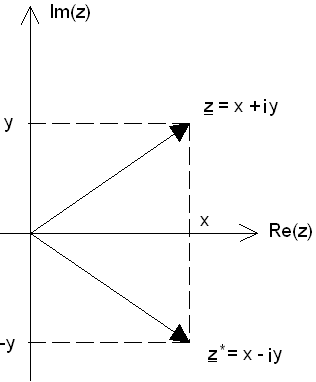
\includegraphics[width=4cm]{images/komplexe_zahlen.png}
\end{minipage}

\subsection{Euler-Formeln} 
$\cos{\alpha}+\im \sin{\alpha} = cjs(\alpha)= \e^{\im \alpha}$\\
$\cos{\alpha}-\im \sin{\alpha} = -cjs(\alpha)= \e^{-\im \alpha}$

\begin{tabbing}
		xxxxxxxxxxxxxxxx \= xxxxxxxxxxxxxxxx \= xxxxxxxxxxxxxxxx \=\kill
		$\sin{\alpha}=\frac{\e^{\im\alpha}-\e^{-\im\alpha}}{2\im}$\> $\cos{\alpha}=\frac{\e^{\im\alpha}+\e^{-\im\alpha}}{2}$\>$\tan{\alpha}=\frac{\sin{\alpha}}{\cos{\alpha}}$\>$\cot{\alpha}=\frac{\cos{\alpha}}{\sin{\alpha}}$
\end{tabbing}